\documentclass{article}
\usepackage[utf8]{inputenc}
\usepackage{graphicx}
\graphicspath{ {./src/} }
\usepackage[dvipsnames]{xcolor}
\usepackage{hyperref}
\hypersetup{colorlinks=true, linkcolor=cyan, urlcolor=orange}
\usepackage[font=footnotesize]{caption}
\usepackage{amsmath}
\usepackage{circledsteps}
\usepackage{xspace}

\usepackage{xspace}

\newcommand{\TODO}[1]{\textcolor{red}{TODO: #1}}
\newcommand{\original}[1]{\textcolor{brown}{#1}}
\newcommand{\perturbed}[1]{\textcolor{teal}{#1}}
\newcommand{\correct}[1]{\textcolor{teal}{#1}}
\newcommand{\wrong}[1]{\textcolor{purple}{#1}}
\newcommand{\correcteq}{$\textcolor{teal}{\checkmark}$}
\newcommand{\wrongeq}{$\textcolor{purple}{\times}$}
\newcommand{\tabincell}[2]{\begin{tabular}{@{}#1@{}}#2\end{tabular}}
\newcommand{\perfdrop}[2]{#1\% absolute drop and #2\% relative drop}
\newcommand{\perfimprove}[2]{#1\% absolute improvement and #2\% relative improvement}

\newcommand{\refequ}[1]{Equation~(\ref{#1})}
\newcommand{\reffig}[1]{Figure~\ref{#1}}
\newcommand{\refsec}[1]{\S\ref{#1}} % \textsection
\newcommand{\reftab}[1]{Table~\ref{#1}}
\newcommand{\refdef}[1]{Definition~\ref{#1}}
\newcommand{\refalgo}[1]{Algorithm~\ref{#1}}
\newcommand{\refapp}[1]{Appendix~\ref{#1}}


\def\eg{\textit{e.g.}\xspace}
\def\Eg{\textit{E.g.}\xspace}
\def\etal{\textit{et al.}\xspace}
\def\etc{\textit{etc.}\xspace}
\def\ie{\textit{i.e.}\xspace}
\def\Ie{\textit{I.e.}\xspace}
\def\vs{\textit{vs.}\xspace}
\def\wrt{\textit{w.r.t.}\xspace}


\begin{document}

\begin{titlepage}
    \begin{center}
            
        \Large
        \textbf{ECE 385: Digital Systems Laboratory}
            
        \vspace{0.2cm}
        % \Large
        Fall 2022
        
        \vspace{0.2cm}
        Final Project

        % \vspace{1.5cm}
        \vfill
        
        \Huge
        \textbf{Final Project Proposal \textit{Tower of the Sorcerer}}
            
        \vfill
            
        \Large
        Jialiang Xu (jx17)\\
        Jinrui Hu (jinruih2)\\
        TA: Neo Yuan\\
        \today
            
    \end{center}
\end{titlepage}

\section{Introduction}
% Summarize the basic functionality of the multiplier circuit

In this report, we describe the multiplier circuit that is capable of conducting multiplication between two 8-bit 2's complement numbers. 

The multiplier is consisted of two 8-bit registers $A$ and $B$, one 1-bit register $X$, 8-bit switches $S$, four 7-segment $Hex$ displays, and two buttons \Circled{Run} and \Circled{Load-Clear-Reset}. 

To conduct the multiplication operation, the \texttt{multiplicand} is first set on the switches, and then loaded into the register $B$ when \Circled{Load-Clear-Reset} is pushed and released. The \texttt{multiplier} is set and stays on the switches $S$. When the \Circled{Run} button is pushed, the final 16-bit result will be computed. It will be stored in registers $AB$ and displayed on the $Hex$ displays. The multiplier also supports consecutive multiplication, which uses the previous result as the multiplicand in the next round of calculation.

In the rest of this report, multiple aspects relevant to the multiplier are covered. We start off with answering the pre-lab question in \refsec{sec:pre-lab}. Then, the written description and diagrams of the multiplier circuit are provided in \refsec{sec:written-description}.


\section{Pre-Lab Question}
\label{sec:pre-lab}
In this section we answer the question asked in the pre-lab part of the Experiment \#4 manual\footnote{See \url{https://wiki.illinois.edu/wiki/display/ECE385FA22/Lab+4}}.

\textbf{Question:} Rework the multiplication example on page 5.2 of the lab manual, as in compute 11000101 * 00000111 in a table like the example. Note that the order of the multiplicand and multiplier are reversed from the example.

\textbf{Answer:} Initial Values: X = 0, A = 00000000, B = 11000101 (achieved using ClearA\_LoadB signal), S = 00000111, M is the least significant bit of the multiplier (Register B). The calculating process can be found in \reftab{tab:pre-lab}.

\begin{table}[h]
    \resizebox{\textwidth}{!}{%
    \begin{tabular}{|l|c|c|c|c|l|}
    \hline
    Function                                                            & X & A         & B                         & M & Comments for   the next step                                                                                           \\ \hline
    \begin{tabular}[c]{@{}l@{}}Clear A, \\ LoadB, \\ Reset\end{tabular} & 0 & 0000 0000 & \textit{00000111}         & 1 & \begin{tabular}[c]{@{}l@{}}Since   M = 1, multiplicand (available from \\ switches S) will be added to A.\end{tabular} \\ \hline
    ADD                                                                 & 1 & 1100 0101 & \textit{00000111}         & 1 & Shift XAB by one bit   after ADD complete                                                                              \\ \hline
    SHIFT                                                               & 1 & 1110 0010 & 1 \textit{0000011}        & 1 & Add S to A since M =   1                                                                                               \\ \hline
    ADD                                                                 & 1 & 1010 0111 & 1 \textit{0000011}        & 1 & Shift XAB by one bit   after ADD complete                                                                              \\ \hline
    SHIFT                                                               & 1 & 1101 0011 & 11 \textit{000001}        & 1 & Add S to A since M =   1                                                                                               \\ \hline
    ADD                                                                 & 1 & 1001 1000 & 11 \textit{000001}        & 1 & Shift XAB by one bit   after ADD complete                                                                              \\ \hline
    SHIFT                                                               & 1 & 1100 1100 & 011 \textit{00000}        & 0 & Do not add S to A   since M = 0. Shift XAB.                                                                            \\ \hline
    SHIFT                                                               & 1 & 1110 0110 & 0011 \textit{0000}        & 0 & Do not add S to A   since M = 0. Shift XAB.                                                                            \\ \hline
    SHIFT                                                               & 1 & 1111 0011 & 00011 \textit{000}        & 0 & Do not add S to A   since M = 0. Shift XAB.                                                                            \\ \hline
    SHIFT                                                               & 1 & 1111 1001 & 100011 \textit{00}        & 0 & Do not add S to A   since M = 0. Shift XAB.                                                                            \\ \hline
    SHIFT                                                               & 1 & 1111 1100 & 1100011 \textit{0}        & 0 & Do not add S to A   since M = 0. Shift XAB.                                                                            \\ \hline
    SHIFT                                                               & 1 & 1111 1110 & 01100011                  & 1 & 8$^{th}$ shift done. Stop.   16-bit Product in AB.                                                                          \\ \hline
    \end{tabular}}
    \caption{The Calculating Process of ``11000101 $\times$ 00000111'' by the Multiplier Circuit}
    \label{tab:pre-lab}
    \end{table}
    


\section{Written Description and Diagrams of Multiplier Circuit}
\label{sec:written-description}

\subsection{Summary of Operation}
% Explain in words how operands are loaded, how the multiplier computes its result, how the result is stored, etc.
The operation has three major stages: 1) the operands being loaded, 2) the multiplier computing the result, and 3) the result being stored and displayed.

To load the operands, the \texttt{multiplicand} is first set on the switches, and then loaded into the register $B$ when \Circled{Load-Clear-Reset} is pushed and released. This is done by connecting the \texttt{Load} port of register $B$ to the signal generated by the button. The \texttt{multiplier} is set and stays on the switches $S$. 

To compute the result, the multiplier utilizes a \texttt{Finite State Machine}, an \texttt{Add/Subtract} module, and a \Circled{Run} button. When the button is pushed, the \texttt{Finite State Machine} starts transitioning and generating control signals according to the given multiplication algorithm. The \texttt{Add/Subtract} module takes in the control signals, carries out the algorithm by adding to / subtracting from the shift registers.

To store and display the result is a trivial process. When the final 16-bit result is computed, it resides in the concatenation of the registers $AB$ which is connected to the $Hex$ display digits. 

The multiplier also supports consecutive multiplication, which uses the previous result as the multiplicand in the next round of calculation. This is achieved naturally with the design of the multiplier described above. Note that the result will be truncated into 8-bits when regarded as an operand, so when the result is higher than 8-bit this feature will be malfunctioning.


\subsection{Top Level Block Diagram}
% This can be generated from the RTL viewer. Please only include the top-level diagram and not the RTL view of every module

\begin{figure}[h]
    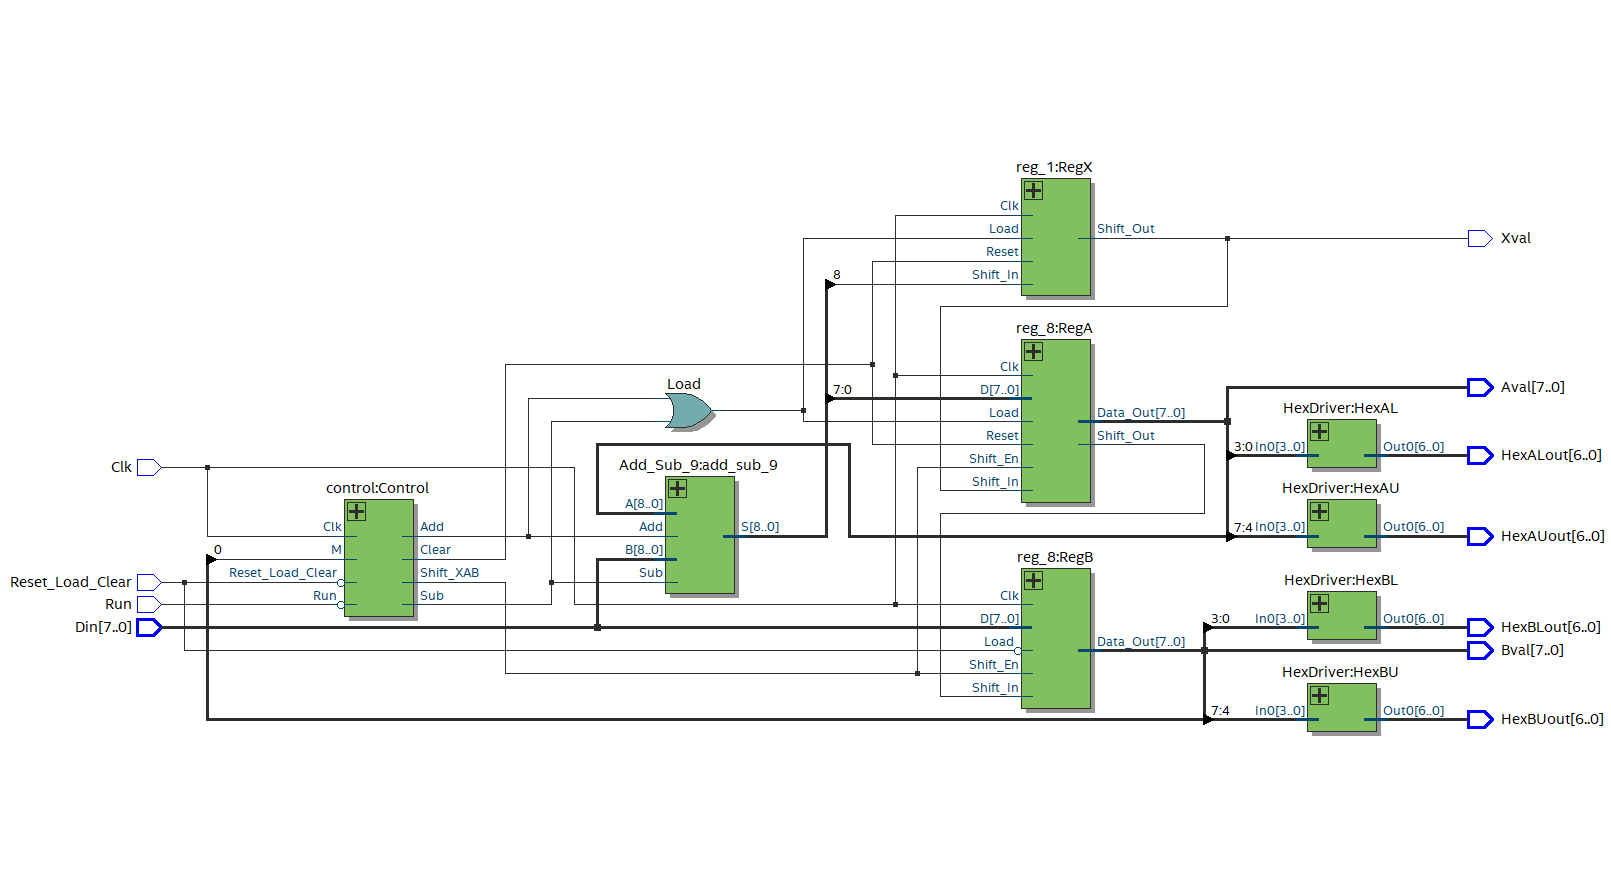
\includegraphics[width=0.9\textwidth]{src/top_level.png}
    \caption{The Top Level Block Diagram of the Multiplier.}
    \label{fig:top_level}
\end{figure}

The top level block diagram can be found in \reffig{fig:top_level}. From left to right there are four major components of the circuit: 
\begin{itemize}
    \item The \texttt{Control} module that generates control signals which are utilized by other components.
    \item The \texttt{Add/Subtract} module that takes in control signals and manipulate register values accordingly.
    \item The \texttt{Register} module that load and stores operands, intermediate values, and final compuation results.
    \item The \texttt{Display} module that consists of four $Hex$ displays connected to Register $A$ and $B$ for displaying register values.
    
\end{itemize}


\subsection{Written Description of .sv Modules}
% \begin{itemize}
%     \item List all modules used in a format shown in the appendix of this document
%     \item You may insert expanded RTL diagrams of each individual module here if it is legible.
% \end{itemize}

\subsubsection{The \texttt{Control} module}
\begin{figure}[h]
    \centering
    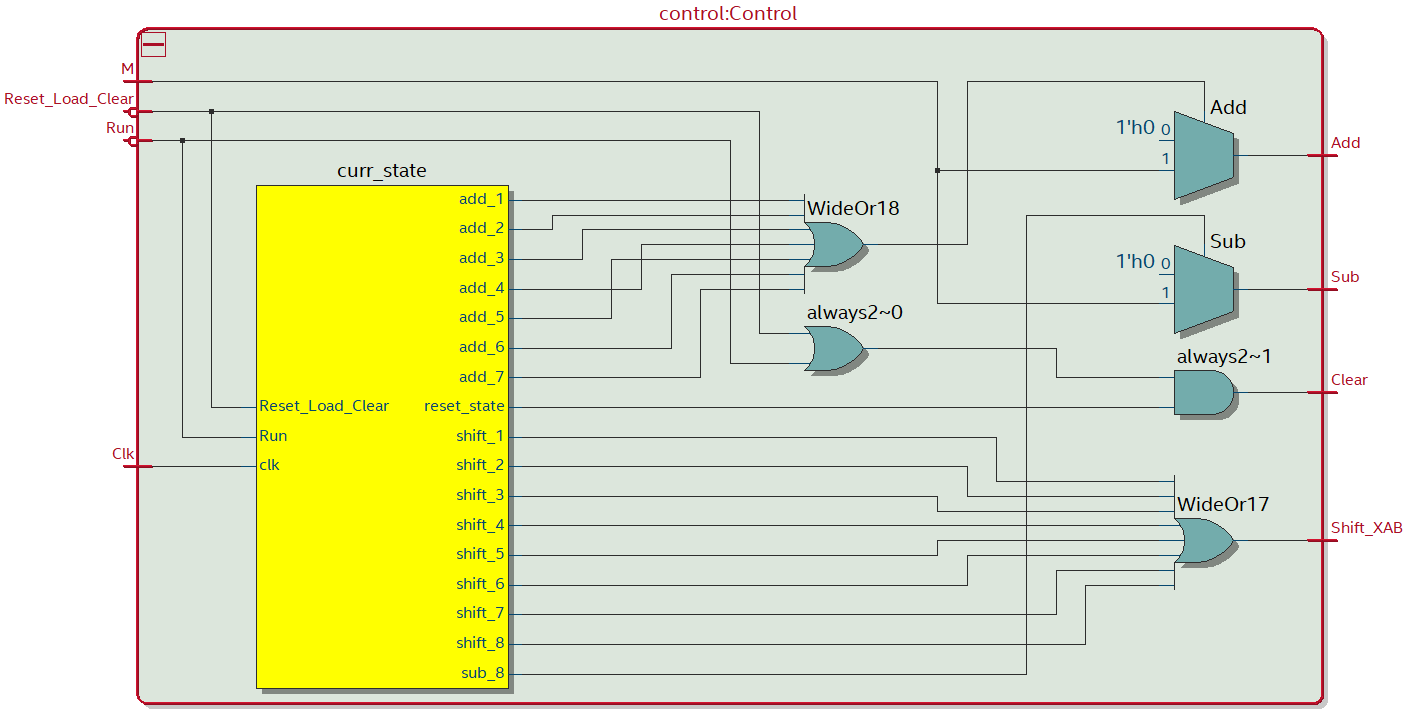
\includegraphics[width=\textwidth]{control.png}
    \caption{The Block Diagram of the Control Module}
    \label{fig:control}
\end{figure}

\begin{itemize}
    \item \textbf{Module:} \texttt{control} in control.sv
    \item \textbf{Inputs:} Clk, Reset\_Load\_Clear, Run, M
    \item \textbf{Outputs:} Shift\_XAB, Add, Sub, Clear
    \item \textbf{Description:} This module keeps track of the current circuit status with an \texttt{Finite State Machine}. At each state, the \texttt{control} module generates signals that will determine the behavior of the connected \texttt{Add\_Sub\_9} and \texttt{reg\_8} modules (see \reffig{fig:top_level} for connection details). 
    \item \textbf{Purpose:} to control the circuit behavior by keeping track of the circuit status and generating control signals.
\end{itemize}


\subsubsection{The \texttt{FullAdder} module}
\begin{figure}[h]
    \centering
    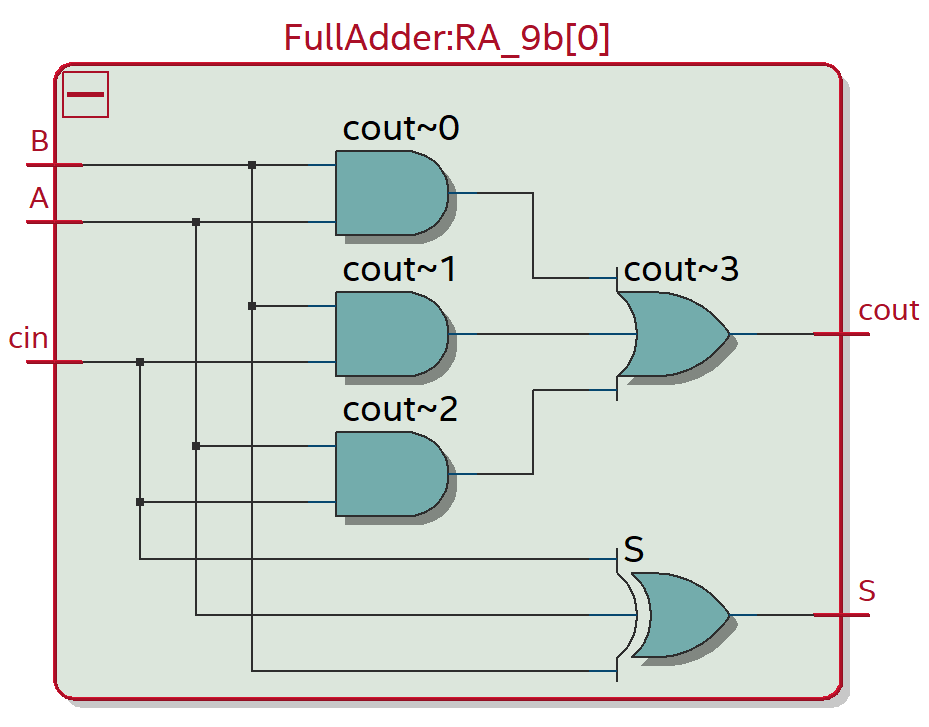
\includegraphics[width=0.5\textwidth]{full_adder.png}
    \caption{The Block Diagram of the FullAdder Module}
    \label{fig:full_adder}
\end{figure}

\begin{itemize}
    \item \textbf{Module:} \texttt{FullAdder} in Adder.sv
    \item \textbf{Inputs:} A, B, cin
    \item \textbf{Outputs:} S, cout
    \item \textbf{Description:} This module performs simple full adding functionality.
    \item \textbf{Purpose:} to facilitate the building of the higher-level 8-bit ripple adder.
\end{itemize}


\subsubsection{The \texttt{RippleAdder} module}
\begin{figure}[h]
    \centering
    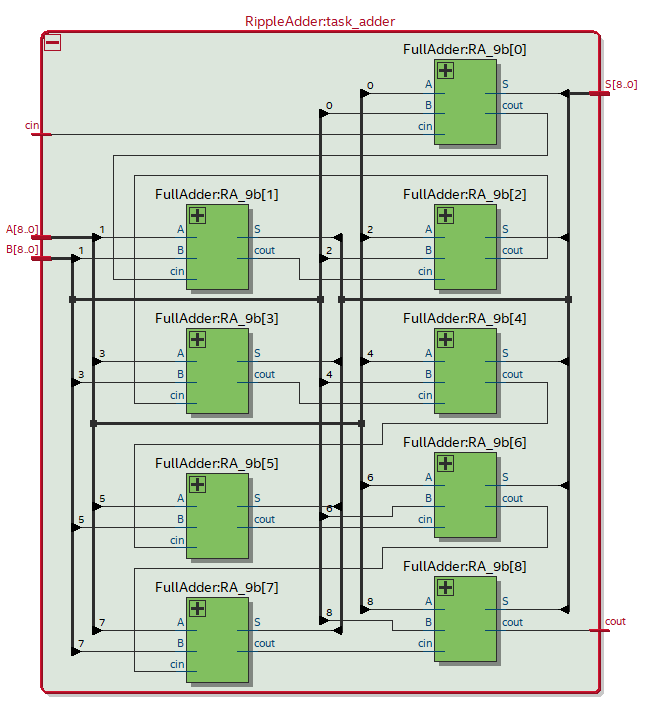
\includegraphics[width=0.45\textwidth]{ripple_adder.png}
    \caption{The Block Diagram of the RippleAdder Module}
    \label{fig:ripple_adder}
\end{figure}

\begin{itemize}
    \item \textbf{Module:} \texttt{RippleAdder} in Adder.sv
    \item \textbf{Inputs:} [8:0] A, [8:0] B, cin
    \item \textbf{Outputs:} [8:0] S, cout
    \item \textbf{Description:} This module performs adding by rippling the simply passing the carry bit across eight full adder modules, as decribed in the previous Experiment\footnote{\url{https://wiki.illinois.edu/wiki/display/ECE385FA22/Lab+3}}.
    \item \textbf{Purpose:} to facilitate building the higher-level \texttt{Add/Subtract} module.
\end{itemize}


\subsubsection{The \texttt{Add/Subtract} module}
\begin{figure}[h]
    \centering
    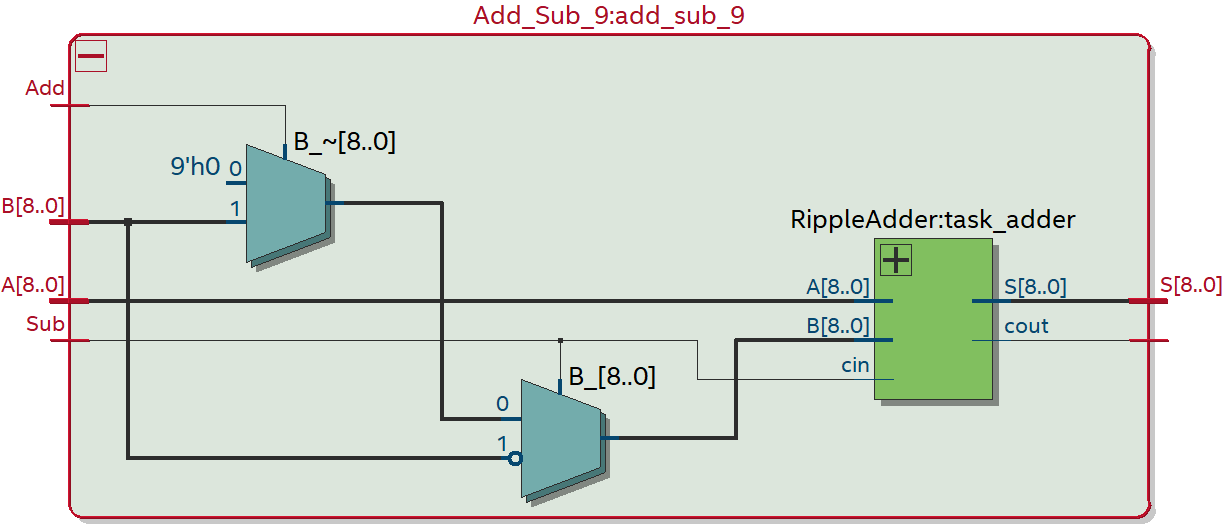
\includegraphics[width=0.8\textwidth]{add_sub.png}
    \caption{The Block Diagram of the Add/Subtract Module}
    \label{fig:add_sub}
\end{figure}

\begin{itemize}
    \item \textbf{Module:} \texttt{Add\_Sub\_9} in Adder.sv
    \item \textbf{Inputs:} [8:0] A, [8:0] B, Add, Sub
    \item \textbf{Outputs:} [8:0] S, cout
    \item \textbf{Description:} during the computation of the multiplication, every time the last bit of Register $B$ (also referred to as $M$) is a logic one, the module adds the \texttt{Multiplicand} on $S$ to $A$ except when it is in the last cycle of the SHIFT-ADD/SUB repetition of the \texttt{Finite State Machine} where it subtracts $S$ from $A$ instead. This behavior utilizes the control signals generated by the \texttt{Control} module.
    \item \textbf{Purpose:} this module conducts the specific multiplication process between the Register $A$ and the switches $S$. It performs adding or subtracting based on the output of the \texttt{Control} module. 
\end{itemize}

\clearpage


\subsubsection{The \texttt{reg\_1} module}
\begin{figure}[h]
    \centering
    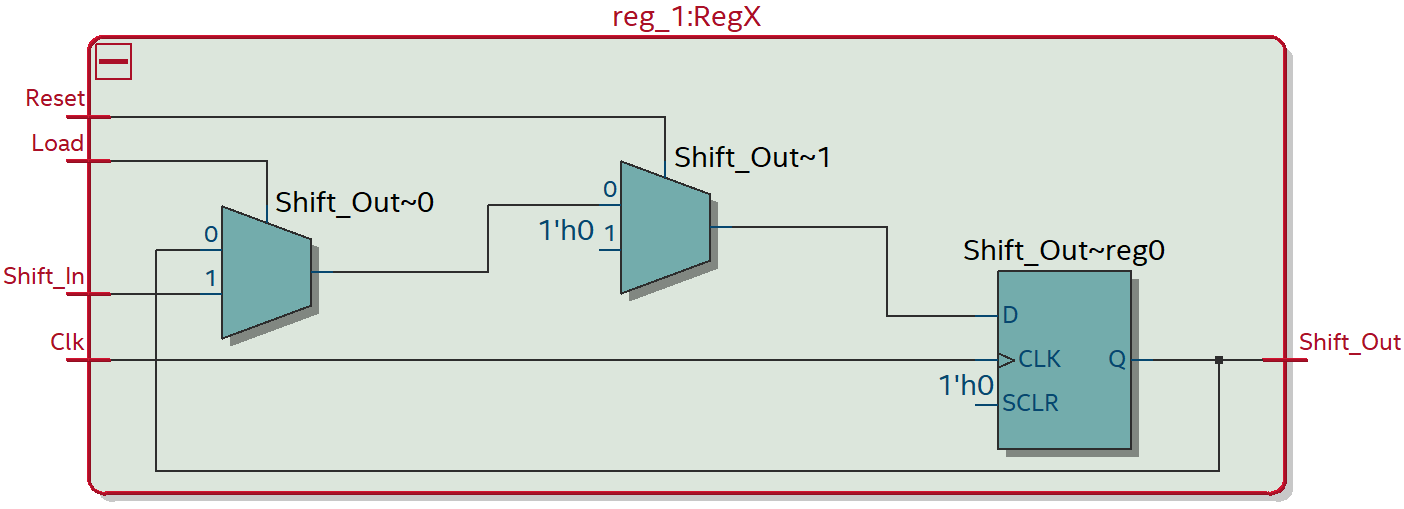
\includegraphics[width=0.8\textwidth]{reg_1.png}
    \caption{The Block Diagram of the reg\_1 Module}
    \label{fig:reg_1}
\end{figure}

\begin{itemize}
    \item \textbf{Module:} \texttt{reg\_1} in reg\_8.sv
    \item \textbf{Inputs:} Clk, Reset, Shift\_In, Load
    \item \textbf{Outputs:} Shift\_Out
    \item \textbf{Description:} a simple 1-bit shift register used to load and store values participating in the compuation process.
    \item \textbf{Purpose:} this module is used to implement the Register $X$ for sign extension during the arithmetic shifting in the computation process.
\end{itemize}


\subsubsection{The \texttt{reg\_8} module}
\begin{figure}[h]
    \centering
    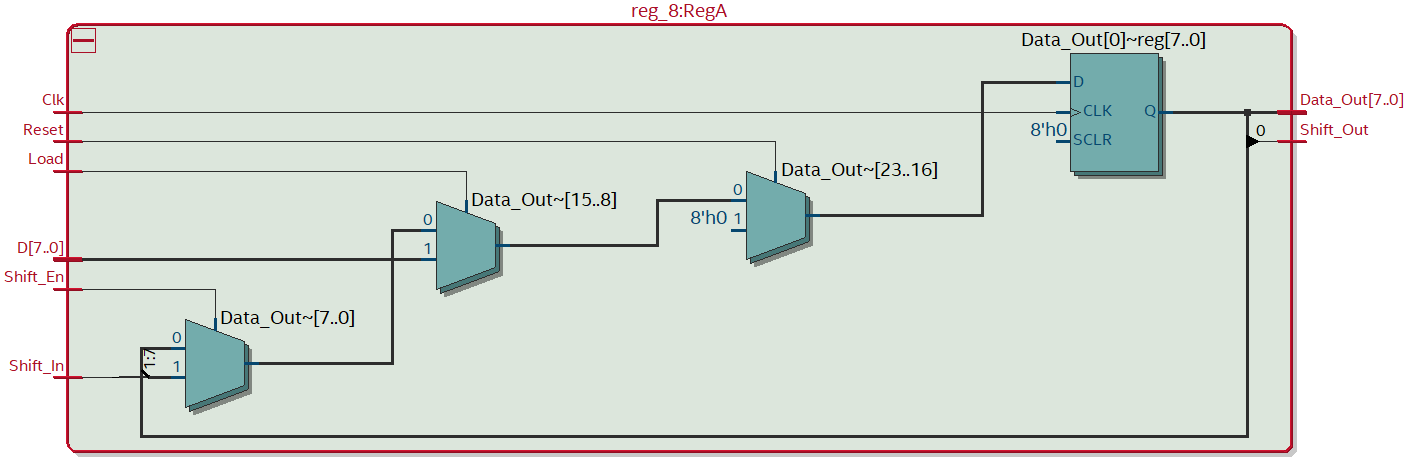
\includegraphics[width=\textwidth]{reg_8.png}
    \caption{The Block Diagram of the reg\_8 Module}
    \label{fig:reg_8}
\end{figure}

\begin{itemize}
    \item \textbf{Module:} \texttt{reg\_8} in reg\_8.sv
    \item \textbf{Inputs:} [7:0] D, Clk, Reset, Shift\_In, Load, Shift\_En
    \item \textbf{Outputs:} [7:0] Data\_Out, Shift\_Out
    \item \textbf{Description:} a simple 8-bit shift register used to load and store values participating in the compuation process.
    \item \textbf{Purpose:} this module is used to implement the Registers $A$, $B$ for loading and storing the to-be-computed values of the \texttt{Multiplicand} and \texttt{Multiplier}. The concatenation of Registers $A$ and $B$ are also used to display the final computed result.
\end{itemize}


\subsubsection{The \texttt{HexDriver} module}
\begin{figure}[h]
    \centering
    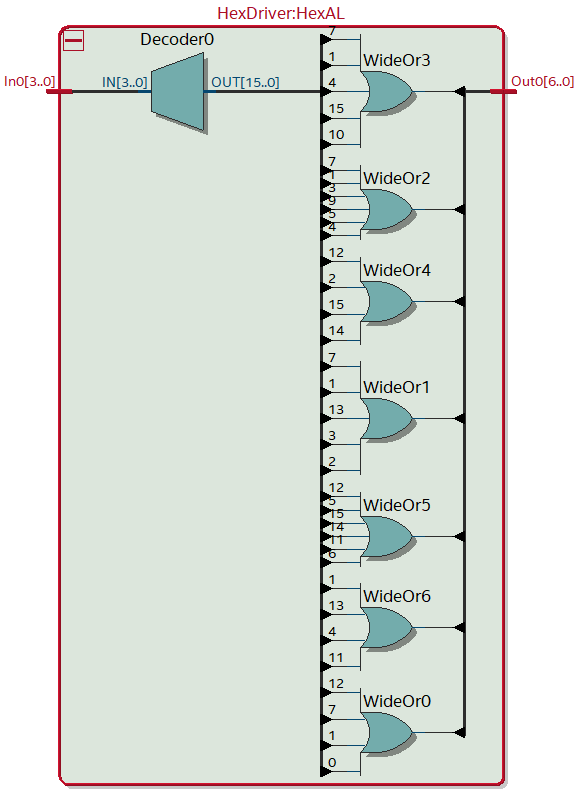
\includegraphics[width=0.5\textwidth]{hex_driver.png}
    \caption{The Block Diagram of the HexDriver Module}
    \label{fig:hex_driver}
\end{figure}

\begin{itemize}
    \item \textbf{Module:} \texttt{reg\_8} in reg\_8.sv
    \item \textbf{Inputs:} Clk, Reset, Shift\_In, Load
    \item \textbf{Outputs:} Shift\_Out
    \item \textbf{Description:} a simple Hex Display driver that outputs corresponding 7-bit signals that interprets a 4-bit binary value into human-readable hexadecimal outputs.
    \item \textbf{Purpose:} this module is used to visualize the values stored in the Registers $A$, $B$ so that the operands and compuation results can be read from the display directly for human evaluation.
\end{itemize}


\subsection{State Diagram for Control Unit}
% This can be done in a program like Visio, but if the Quartus state diagram generator is used, you must label the states and transitions. By default, the tool does not generate a very legible state diagram.
\begin{figure}[h]
    \centering
    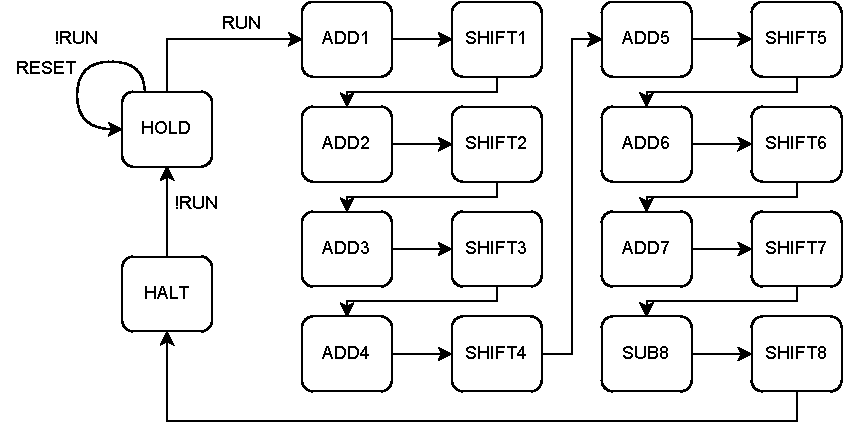
\includegraphics[width=0.8\textwidth]{fsm_chart.pdf}
    \caption{The State Diagram of the Finite State Machine in the Control Module. }
    \label{fig:state}
\end{figure}

At the state ``SUB8'' or states with names of the shape ``ADD\#'', the control signals depend on the last bit of Register $B$ (\ie, $M$). When $M$ is a logical one, $Shift = 1$, $Add = 1$, $Sub = 0$ for ``ADD\#'' and $Shift = 1$, $Add = 0$, $Sub = 1$ for ``SUB8'', otherwise $Shift = 0$, $Add = 0$, $Sub = 0$.

At the states with names of the shape ``SHIFT\#'', the control signals generated will be $Shift = 1$, $Add = 0$, $Sub = 0$.


\section{Annotated Pre-Lab Simulation Waveforms}
% \begin{itemize}
%     \item Must show 4 operations where operands have signs (+*+), (+*-), (-*+) and (-*-)
%     \item Waveform must have notes that clearly show the operands as well as the result, etc
% \end{itemize}

\begin{figure}[h]
    \centering
    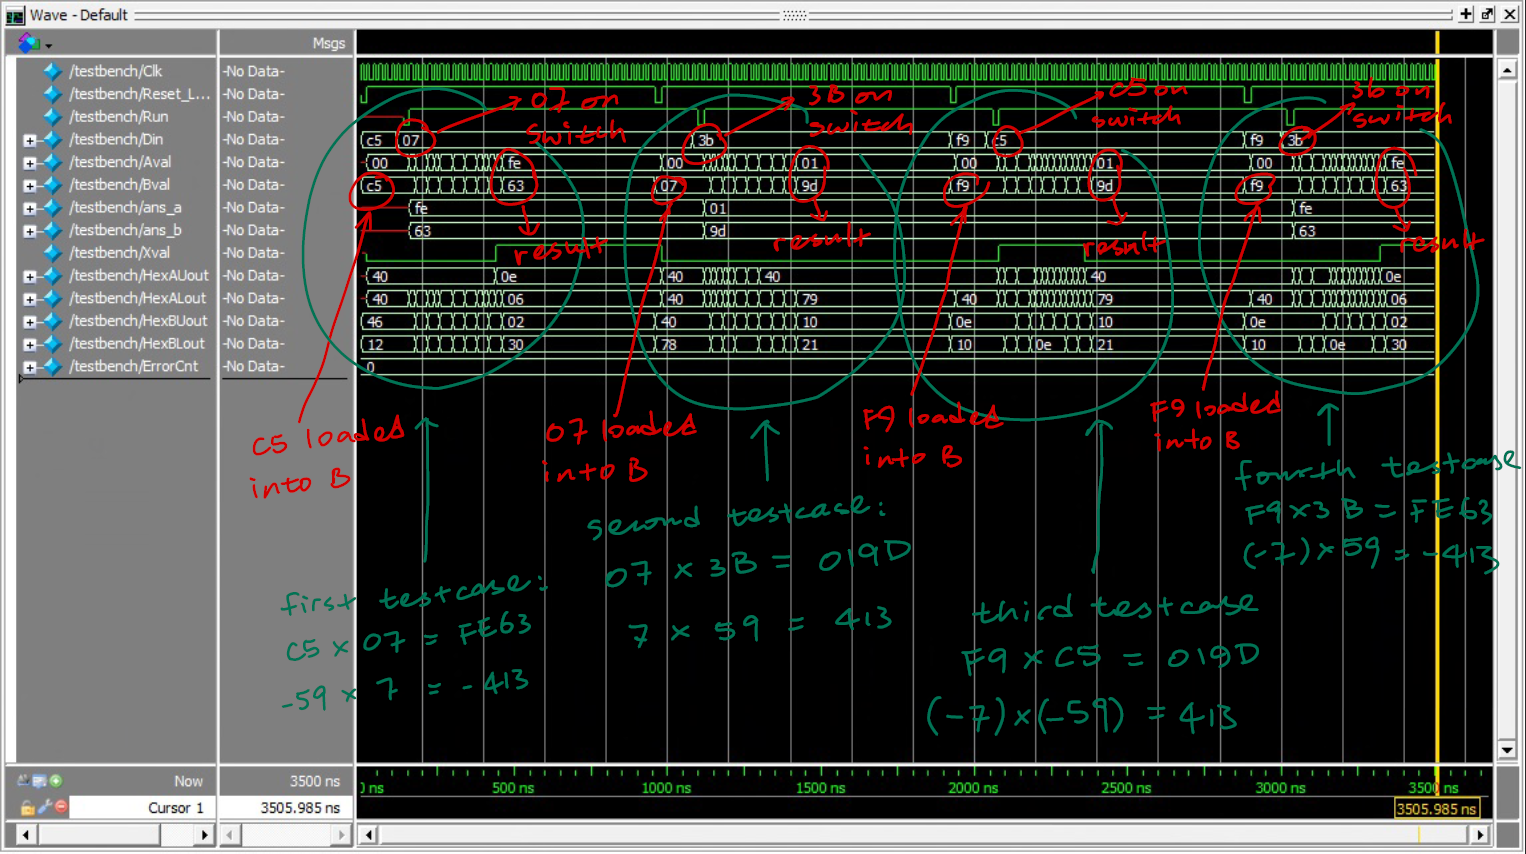
\includegraphics[width=\textwidth]{annotated.png}
    \caption{The Annotated Pre-Lab Simulation Waveforms}
\end{figure}

\clearpage


\section{Answers to Post-Lab Questions}
% \begin{itemize}
%     \item Fill in the table shown in 5.6 with your design’s statistics
%     \item Answer all the post-lab questions. As usual, they may be in their own section or dispersed into the appropriate sections in the rest of the report.
% \end{itemize}
In this section we answer the questions in the Post-Lab section of the Experiment manual. The order is determined by the questions' order in the manual.

\subsection{Compilation Report Table}
\begin{table}[h]
    \centering
    \begin{tabular}{|c|c|}
    \hline
    LUT           & 102                    \\ \hline
    DSP           & N/A                    \\ \hline
    Memory (BRAM) & 0 / 1,677,312 ( 0 \% ) \\ \hline
    Flip-Flop     & 0                      \\ \hline
    Frequency     & 204.37 MHz             \\ \hline
    Static Power  & 90.05 mW               \\ \hline
    Dynamic Power & 0.00 mW                \\ \hline
    Total Power   & 121.81 mW              \\ \hline
    \end{tabular}
    \caption{The Resource Usage Table of the Circuit}
    \label{tab:resource_usage}
\end{table}

To optimize the design's maximum frequency, we can switch from the Carry Ripple Adder to a Carry Select Adder, so that the latency for the addition or subtraction can be reduced.

\subsection{Written Questions}
In this section we answer the questions that requires a written response proposed in the Post-Lab section.

\subsubsection{What is the purpose of the X register? When does the X register get set/cleared?}
The purpose of the Register $X$ in our design is to enable arithmetic shift during the computation, which keeps the value's sign bit when conducting right-shifting. Register $X$ is critical because it keeps track of the sign bit of Register $A$, which will be placed as the new most significant bit after a shift on Register $A$ has been finished.


\subsubsection{What would happen if you used the carry out of an 8-bit adder instead of output of a 9-bit adder for X?}
If the carry out of an 8-bit adder is used instead, the behavior will be incorrect. Under cases where a negative result does not generate a carry out (\eg, -1d + 0d), or where a positive result generates a carry out (\eg, -1d + 2d), the carry out cannot correctly reflect the sign bit of the final result and will lead to erroneous behavior.


\subsubsection{What are the limitations of continuous multiplications? Under what circumstances will the implemented algorithm fail?}
Between two runs of the multiplication, the Register $A$ and $X$ will be cleared since they will be used to hold data in the compuation process. This leads to the behavior that the result will be truncated to the length same to that of Register $B$, which is 8 bits. This will not be an issue when the final result's value is persisted after the truncation, however when the absolute value of the number is larger than a threshold (in our case, $\geq 256d$ or $\leq -256d$), the result will be incorrect and the continuous multiplication will fail.


\subsubsection{What are the advantages (and disadvantages?) of the implemented multiplication algorithm over the pencil-and-paper method discussed in the introduction?}


\begin{itemize}
    \item \textbf{Advantages}: it is making full use of the shift register where each bit of the registers is taking a piece of working information during each time step of the process, thus it avoids wasting hardware resources on the FPGA, comparing to the pencil-and-paper algorithm where the storage and summation of eight 16-bit intermediate result are needed.
    
    \item \textbf{Disadvantages}: the algorithm itself is less intuitive, and the implementation is less straightforward.
\end{itemize} 


\section{Conclusion}
% \begin{itemize}
%     \item Discuss functionality of your design. If parts of your design did not work, discuss what could be done to fix it.
%     \item Was there anything ambiguous, incorrect, or unnecessarily difficult in the lab manual or given materials which can be improved for next semester? You can also specify what we did right, so it does not get changed.
% \end{itemize}
\subsection{Functionality Discussion}
In this experiment, we implemented the Multiplier circuit capable of conducting multiplication between two 8-bit 2's complement numbers. 

To conduct the multiplication operation, the \texttt{multiplicand} is first set on the switches, and then loaded into the register $B$ when \Circled{Load-Clear-Reset} is pushed and released. The \texttt{multiplier} is set and stays on the switches $S$. When the \Circled{Run} button is pushed, the final 16-bit result will be computed. It will be stored in registers $AB$ and displayed on the $Hex$ displays. The multiplier also supports consecutive multiplication, which uses the previous result as the multiplicand in the next round of calculation.


\subsection{Lab Manual Suggestions}
The lab manuals are of high-quality, they are clear, easy to follow, and have very few things that can be better. One such thing is that the indexing can be more consistent. For instance the title of the manual pdf itself says Experiment 8 which is not true, and on page 5.8 it says ``fill in the table shown on 5.6 with your design's statistics'', but the table is on page 4.7.

\end{document}
